% This file requires figure.pdf and it should be processed by pdflatex.

%%%%%%%%%%%%%%%%%%%%%%%%%%%%%%%%%%%%%%%%%%%%%%%%%%%%%%%%%%%%%%%%%%%%%
%%           Topology Proceedings Sample Latex Article             %%
%%%%%%%%%%%%%%%%%%%%%%%%%%%%%%%%%%%%%%%%%%%%%%%%%%%%%%%%%%%%%%%%%%%%%

\documentclass{amsart}
\usepackage[T1]{fontenc}   %%%%%%%Please do not change
\usepackage{graphics}                  %%%%%%%

\usepackage{amsmath}
\usepackage{amsthm}
\usepackage{amssymb}

\usepackage{graphicx}

%%%%%%%%%%%%%%%%%%%%%%%%%%%%%%%%%%%%%%%%%%%%%%
%%%%%%%%%%%%%%%%%%%%%%%%%%%%%%%%%%%%%%%%%%%%%%
% Please do not change this paragraph. %%%%%%%
\setcounter{page}{1}                   %%%%%%%
\setlength{\textwidth}{4.4in}          %%%%%%%
\setlength{\textheight}{7.0in}         %%%%%%%
\setlength{\evensidemargin}{1in}       %%%%%%%
\setlength{\oddsidemargin}{1in}        %%%%%%%
\setlength{\topmargin}{.8in}           %%%%%%%
%%%%%%%%%%%%%%%%%%%%%%%%%%%%%%%%%%%%%%%%%%%%%%
%%%%%%%%%%%%%%%%%%%%%%%%%%%%%%%%%%%%%%%%%%%%%%
% Please do not change the page size   %%%%%%%
% and do not redefine the baselineskip.%%%%%%%
%%%%%%%%%%%%%%%%%%%%%%%%%%%%%%%%%%%%%%%%%%%%%%
%%%%%%%%%%%%%%%%%%%%%%%%%%%%%%%%%%%%%%%%%%%%%%


\newtheorem{theorem}{Theorem}[section]
\newtheorem{proposition}[theorem]{Proposition}
\newtheorem{lemma}[theorem]{Lemma}
\newtheorem{corollary}[theorem]{Corollary}


\theoremstyle{definition}
\newtheorem{definition}[theorem]{Definition}
\newtheorem{example}[theorem]{Example}
\newtheorem{question}[theorem]{Question}




\begin{document}

%%%%%%%%%%%%%%%%%%%%%%%%%%%%%%%%%%%%%%%%%%%%%%%%%%%%%%%%%%%%
%%%%%%%%%%%%%%%%%%%%%%%%%%%%%%%%%%%%%%%%%%%%%%%%%%%%%%%%%%%%
% This a placeholder for the TOPLOGY PROCEEDINGS logo %%%%%%
\noindent                                             %%%%%%
\begin{picture}(150,36)                               %%%%%%
\put(5,20){\tiny{Submitted to}}                       %%%%%%
\put(5,7){\textbf{Topology Proceedings}}              %%%%%%
\put(0,0){\framebox(140,34){}}                        %%%%%%
\put(2,2){\framebox(136,30){}}                        %%%%%%
\end{picture}                                        %%%%%%
%%%%%%%%%%%%%%%%%%%%%%%%%%%%%%%%%%%%%%%%%%%%%%%%%%%%%%%%%%%%
%%%%%%%%%%%%%%%%%%%%%%%%%%%%%%%%%%%%%%%%%%%%%%%%%%%%%%%%%%%%
\vspace{0.5in}


\renewcommand{\bf}{\bfseries}
\renewcommand{\sc}{\scshape}
\newcommand{\<}{\langle}
\renewcommand{\>}{\rangle}
%insert defs/styles
\vspace{0.5in}


\title[Destruction of metrizability in generalized inverse limits]%
{Destruction of metrizability in generalized inverse limits}

%    Information for first author:
\author{Steven Clontz}
\address{Department of Mathematics and Statistics, Fretwell Hall, UNC Charlotte, NC 28223}
%    Current address (if needed):
%\curraddr{}
\email{steven.clontz@gmail.com}
%\thanks{}


%    Information for second author (if needed):
\author{Scott Varagona}
\address{Department of Biology, Chemistry \& Mathematics, University of Montevallo,
Montevallo, AL 35115}
\email{svaragona@montevallo.edu}
%\thanks{Support information for the second author.}

%    General info
%%%%%%%%%%%%%%%%%%%%%%%%%%%%%%%%%%%%%%%%%%%%%%%%%%%
\subjclass[2010]{Primary 54F15, 54H20}                                    %
%                                                                                                                           %
%         Please use the current 2010 Mathematics Subject Classification:             %
%         http://www.ams.org/mathscinet/msc/                                                        %
%         http://www.zentralblatt-math.org/msc/en/                                                 %
%%%%%%%%%%%%%%%%%%%%%%%%%%%%%%%%%%%%%%%%%%%%%%%%%%%


\keywords{Inverse Limits, Inverse Limits with set-valued functions, continuum theory, metrizability, idempotent.}
\thanks {}




\begin{abstract}
If $X$ is a compact Hausdorff space, an upper semi-continuous bonding function $f: X \rightarrow 2^{X}$ is said to be idempotent if $f^2 = f$. In this short paper, we prove that if $f: [0,1] \rightarrow C([0,1])$ is u.s.c., idempotent and surjective, but $f$ is not the identity, then the inverse limit with the single bonding function $f$ and with factor spaces indexed by a nonzero ordinal $\kappa$ contains a copy of $\kappa + 1$. It follows that such an inverse limit is only metric in the case where the index set $\kappa$ is countable.
\end{abstract}

\maketitle

\section{Introduction}

As various recent papers have shown (e.g., \cite{char roe}, \cite{varagona}, \cite{vernon}), continuum theorists have begun to broaden their study of generalized inverse limits to the case where the factor spaces are indexed by sets other than the positive integers. This more inclusive approach opens many new avenues for research, and has already produced some interesting results. For example, Patrick Vernon showed that an inverse limit indexed by the set of all integers with a single upper semi-continuous bonding function can be homeomorphic to a 2-cell \cite{vernon}, whereas V. Nall previously showed this is impossible for such an inverse limit indexed by the positive integers alone \cite{nall 2cell}.

In another recent paper \cite{varagona}, S. Varagona generalized many previously known theorems (from, e.g., \cite{ingram mahavier} and \cite{nall connected}) to the case of u.s.c. inverse limits indexed by arbitrary totally ordered sets. As he showed, in that context, inverse limits with a single idempotent upper semi-continuous bonding function become especially important. Relatively little is known about the kind of continua that may be produced by such inverse limits, however.

This short paper focuses on the case of an inverse limit with a single idempotent, surjective, upper semi-continuous, continuum-valued bonding function on $[0,1]$, when the index set of the inverse limit is some nonzero ordinal $\kappa$. In particular, we show that (so long as the bonding function is not the identity) such an inverse limit is metric exactly when $\kappa$ is countable. The strategy, as will be seen, is to show that the inverse limit must contain a copy of $\kappa + 1$.

\section{Background Definitions and Lemmas}

We begin with some useful notation. Let $X$ be a non-empty compact Hausdorff space. Then we denote by $2^X$ the set of all non-empty compact subsets of $X$. We say a subset $A$ of $X$ is a \emph{continuum} if $A$ is non-empty, compact and connected. $C(X)$ denotes the set of all elements of $2^X$ that are continua.

Suppose $X$ and $Y$ are non-empty compact Hausdorff spaces. Then the set-valued function $f: X \rightarrow 2^{Y}$ is said to be \emph{upper semi-continuous} (u.s.c.) at $x \in X$ if, for every open set $V$ in $Y$ with $f(x) \subseteq V$, there exists an open set $U$ in $X$ with $x \in U$ and $f(u) \subseteq V$ for each $u \in U$. If $f$ is u.s.c. at each $x \in X$, we simply say \emph{$f$ is u.s.c.} If $f: X \rightarrow 2^{Y}$ is a set-valued function, then the \emph{graph of $f$}, denoted $G(f)$, is given by $G(f) = \{\langle x , y \rangle \in X \times Y \ | \ y \in f(x)\}$. (Note that, to help distinguish between ordered pairs and intervals on a linearly ordered space, we will use pointed brackets to denote ordered pairs, e.g., $\langle x , y \rangle$, whereas intervals are given in the traditional way with brackets or parentheses, e.g., $(a,b), [c,d]$, etc.) The set-valued function $f: X \rightarrow 2^{Y}$ is said to be \emph{surjective} if, for every $y \in Y$, there exists $x \in X$ with $y \in f(x)$. If a u.s.c. function $f: X \rightarrow 2^{Y}$ has the property that $f(x)$ is connected for each $x \in X$, then $f$ is \emph{continuum-valued}, and we denote this by writing  $f: X \rightarrow C(Y).$ The \emph{identity on} $X$ (also called the \emph{trivial} function on $X$) is the u.s.c. function $\iota$ given by $\iota(x) = \{x\}$ for all $x \in X$; we may simply say the \emph{identity} (or, more simply, $\iota$) when the space $X$ is understood from context.

The following characterization of u.s.c. functions (from \cite{i m paper}) is well-known and often more convenient to work with than the original definition:

\begin{lemma} If $X$ and $Y$ are non-empty compact Hausdorff spaces, then $f: X \rightarrow 2^{Y}$ is u.s.c. if and only if $G(f)$ is closed.
\end{lemma}

If $X$, $Y$, and $Z$ are non-empty compact Hausdorff spaces and $f : X \rightarrow 2^{Y}$ and $g: Y \rightarrow 2^{Z}$ are u.s.c., then the composition $g \circ f : X \rightarrow 2^{Z}$ is the u.s.c. function given by $(g \circ f)(x) = \{z \in Z \ | \ $There exists $y \in Y$ such that $y \in f(x)$ and $z \in g(y)\}$. In the special case where $f: X \rightarrow 2^{X}$, we denote $f \circ f$ by $f^2$. If $f^2 = f$, then we say $f$ is \emph{idempotent}.

Let $\kappa$ be an ordinal. (We follow the convention of set theory in which an ordinal is equal to the set of its predecessors. For more detailed background on ordinals, see, for example, \cite{Kunen}.) Suppose that for each $\alpha \in \kappa$, $X_{\alpha}$ is a non-empty compact Hausdorff space and whenever $\alpha \le \beta \in \kappa$, the set-valued function $f_{\alpha \beta} : X_{\beta} \rightarrow 2^{X_{\alpha}}$ is u.s.c. (With this notation, $f_{\alpha \alpha}$ is always the identity $\iota$ on $X_{\alpha}$.) Suppose further that, whenever $\alpha \le \beta \le \eta \in \kappa$, we have $f_{\alpha \beta} \circ f_{\beta \eta} = f_{\alpha \eta}$. Then the collection $\textbf{f} = \{ f_{\alpha \beta} \ | \ \alpha \le \beta \in \kappa\}$ of u.s.c. functions is said to be \emph{exact}. In this case, we say $\{X_{\alpha}, f_{\alpha \beta}, \kappa\}$ is an \emph{inverse limit system}; the \emph{inverse limit}, $\varprojlim \{X_{\alpha}, f_{\alpha \beta}, \kappa\}$, of this system is $\{ \textbf{x} \in \prod_{\alpha \in \kappa} X_{\alpha} \ | \ x_{\alpha} \in f_{\alpha \beta}(x_{\beta})$ for all $\alpha \le \beta \in \kappa\}$. (In keeping with tradition, a boldface $\textbf{x}$ always denotes an element of $\prod_{\alpha \in \kappa} X_{\alpha}$; the $\alpha$th coordinate of such an $\textbf{x}$ will be denoted $\textbf{x}(\alpha)$.)  We call the u.s.c. functions $f_{\alpha \beta}$ the \emph{bonding functions} of the inverse limit, and each $X_{\alpha}$ is called a \emph{factor space} of the inverse limit.

Because it can be difficult to check if a large collection of u.s.c. functions is exact, a much more tractable case would be that of an inverse limit system with a single idempotent bonding function $f$. That is, suppose $X$ is a non-empty compact Hausdorff space and $f: X \rightarrow 2^{X}$ is an idempotent u.s.c. function. If $X_{\alpha} = X$ for each $\alpha \in \kappa$ and $f_{\alpha \beta} = f$ for each $\alpha < \beta \in \kappa$, then $\{X_{\alpha}, f_{\alpha \beta}, \kappa\} = \{X, f, \kappa\}$ is an \emph{inverse limit system with the single bonding function $f$}, and we denote the inverse limit of the system as $\varprojlim \{X, f, \kappa\}$. (Of course, since $f$ is idempotent, the collection $\textbf{f}$ of bonding functions is automatically exact.) We note that, although the only continuous idempotent surjective function from a compact Hausdorff space $X$ to itself is the identity map, there are many nontrivial examples of u.s.c. idempotent surjective functions on $X$; see Figure \ref{idempotentUsc} for examples.

\begin{figure}
\begin{center}
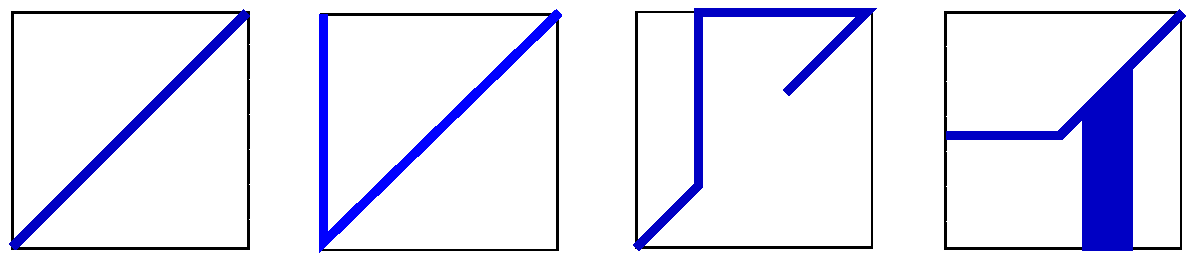
\includegraphics[width=\linewidth]{idempotent_usc.pdf}
\end{center}
\caption{Examples of u.s.c. idempotent surjective functions on [0,1]}
\label{idempotentUsc}
\end{figure}

A detailed study of inverse limits with a single idempotent surjective u.s.c. bonding function was begun in \cite{varagona}. The following is a lemma from that paper which will be used repeatedly (often without being referenced explicitly) in the proofs to come.

\begin{lemma} \label{idemlemma}  Let $X$ be a compact Hausdorff space and let $f: X \rightarrow 2^{X}$ be u.s.c. Then $f$ is idempotent if and only if, whenever $f(x) = A$ for some $x \in X$ and $A \subseteq X$, $f(A) = A$.
\end{lemma}

By applying results by Ingram and Mahavier \cite{ingram mahavier} and by Charatonik and Roe \cite{char roe}, Varagona stated theorems (2.1 and 2.2 in \cite{varagona}) that imply $\varprojlim \{[0,1], f, \kappa\}$ is a continuum when $f$ is u.s.c., idempotent, and continuum-valued (and $\kappa > 0$). On the other hand, Greenwood and Kennedy showed in \cite{greenwood kennedy} that there is a non-continuum-valued u.s.c. surjective idempotent bonding function $f$ (with a connected graph) for which $\varprojlim \{[0,1], f, \omega\}$ is disconnected.

\section{Main Results}

We now focus on the case of an inverse limit with a single idempotent, surjective, u.s.c. bonding function $f: [0,1] \rightarrow C([0,1])$. The main goal of this paper is to prove that if such an $f$ is not the identity and $\kappa$ is a nonzero ordinal, then the inverse limit $\varprojlim \{[0,1], f, \kappa\}$ is metric exactly when the index set $\kappa$ is countable.

Let us say a subset $S$ of $[0,1]^2$ satisfies \textit{condition $\Gamma$} if, for some $x, y \in [0,1]$ with $x \ne y$, $\<x,x\> \in S$, $\<y,y\> \in S$, and either $\<x,y\>$ or $\<y,x\> \in S$; see Figure \ref{conditionGamma}. Let $\Delta = \{\<a,a\> \ | \ a \in [0,1]\}$, and notice that $[0,1]^2 \setminus \Delta$ is the union of two disjoint open sets.

\begin{figure}
\begin{center}
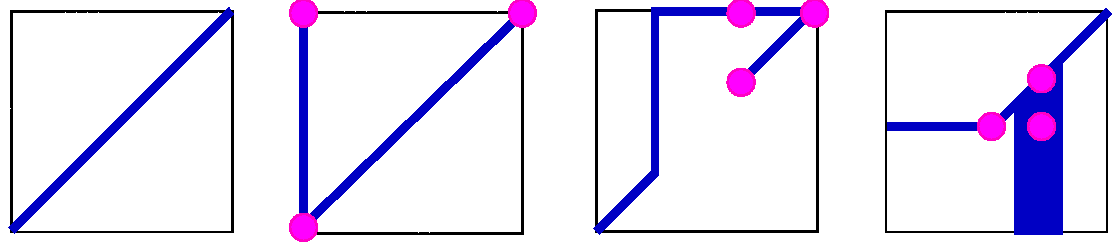
\includegraphics[width=\linewidth]{idempotent_usc_4.pdf}
\end{center}
\caption{Idempotent u.s.c. functions with highlighted points illustrating condition $\Gamma$}
\label{conditionGamma}
\end{figure}

\begin{lemma} \label{first lemma}
If $f: [0,1] \rightarrow C([0,1])$ is u.s.c., then for some $x \in [0,1]$, $\<x,x\> \in G(f)$.
\end{lemma}

\begin{proof}
Suppose that $\<x,x\> \not\in S$ for all $x \in [0,1]$. Then $y > 0$ for all $y \in f(0)$, and $z < 1$ for all $z \in f(1)$. This means $([0,1]^2 \setminus \Delta) \cap G(f) = G(f)$ is the union of two non-empty disjoint open sets. However, since $f$ was continuum-valued and u.s.c., $G(f)$ was connected (by Theorem 2.5 from \cite{ingram intro}), yielding a contradiction.
\end{proof}

\begin{lemma}
If $f: [0,1] \rightarrow C([0,1])$ is u.s.c., idempotent, and surjective, then for some $x, y \in [0,1]$ with $x \not= y$, $\<x,x\> \in G(f)$ and $\<y,y\> \in G(f)$.
\end{lemma}

\begin{proof}
By Lemma \ref{first lemma}, for some $x \in [0,1]$, $\<x,x\> \in G(f)$. Suppose by way of contradiction that, for all $y \in [0,1]$ with $y \not= x$, $\<y,y\> \not\in G(f)$.

\textbf{Case 1:}
$x = 0$. Since $\<1,1\> \not\in G(f)$, it follows that $f(1) \subseteq [0,1)$. It follows then that $f(z)\subseteq[0,z)$ for all $z\in(0,1]$, since $f(z)$ is an interval not containing $z$ and the graph of $f$ is connected. Therefore, as $f$ is surjective and $1 \not\in f(z)$ for all $z \in (0,1]$, $1 \in f(0)$. In fact, as $f(0)$ is connected and contains both $0$ and $1$, we know $f(0) = [0,1]$. Then for $z \in (0,1]$, $f(f(z))=f(z)\subseteq[0,z)\not=[0,1]$, and thus $0\not\in f(z)$, that is, $f(z)\subseteq(0,z)$.

Now consider $f(1)=[a,b]\subseteq(0,1)$, where $a \le b$. (If $a = b$, then $[a,b] = \{a\}$ and the following argument will still apply.) Then $f(f(1))=f([a,b])=[a,b]$, and in particular, $f(a)\subseteq[a,b]$. However, since $a\in(0,1]$, we also have $f(a)\subseteq(0,a)$, a contradiction.


\textbf{Case 2:}
$x = 1$. The proof is analogous to Case 1.


\textbf{Case 3:}
$x \in (0,1)$. Since $f(0) \subseteq (0,1]$ and the graph of $f$ is connected, $f(z) \subseteq (z,1]$ for each $z \in [0,x)$; thus, $0 \not\in f([0,x))$. Likewise,  since $f(1) \subseteq [0,1)$, we have $f(z) \subseteq [0,z)$ for each $z \in (x,1]$; thus, $1 \not\in f((x,1])$. Since $f$ is surjective, $1\in f(v)$ for some $v\in[0,x]$ and $0\in f(w)$ for some $w\in[x,1]$. If $f(v) = \{1\}$, then $f(f(v)) = f(\{1\}) = \{1\}$, which is a contradiction since $\<1,1\> \not\in G(f)$. So, let us say $f(v) = [k,1]$ for some $k < 1$.

We note that in fact, $v=x$. If $v<x$ could hold, then $f(v)=[k,1]\subseteq(v,1]$. Then $f(f(v))=f([k,1])=[k,1]$, which forces $k\leq x$ as $1\not\in f((x,1])$. This results in a contradiction, as then $f([x,1])\subseteq f([k,1])=[k,1]$ while $0\in f(w)\subseteq f([x,1])$. So $[x,1]\subseteq f(x)$, and as $1\not\in f(1)$, we have that $x\not\in f(1)$ by the idempotence of $f$.

So, $f(1) = [a,b]$ for some $a \le b$, where $[a,b] \subseteq [0,x)$ or $[a,b] \subseteq (x,1)$. If $[a,b] \subseteq (x,1)$, then since $a > x$, $f(a) \subseteq [0,a)$ while $f(a)\subseteq f([a,b])=f(f(1))=f(1)=[a,b]$, contradiction. On the other hand, if $[a,b] \subseteq [0,x)$, then since $b<x$, $f(b) \subseteq (b,1]$ while $f(b) \subseteq f([a,b])=f(f(1))=f(1)=[a,b]$, another contradiction. Since each possible case results in a contradiction, the proof is complete.
\end{proof}

\begin{lemma} \label{big lemma}
If $f: [0,1] \rightarrow C([0,1])$ is u.s.c., idempotent, and surjective, but $f \not=\iota$, then $G(f)$ satisfies condition $\Gamma$.
\end{lemma}

\begin{proof}
If $\Delta$ is a subset of $G(f)$, then since $f \not=\iota$, there must exist some point $\<x,y\> \in G(f)$ with $x \not= y$, and the result follows. So, suppose $\Delta$ is not a subset of $G(f)$. The result follows in either of two possible cases.

\textbf{Case 1.} $G(f) \cap \Delta$ is not connected. Then there exist $x<y$ in $[0,1]$ such that $\<x,x\>$ and $\<y,y\>$ are elements of $G(f)$ but for all $p$ with $x < p < y$, $\< p, p \> \not\in G(f)$.

Because $f$ is continuum-valued, we may assume $\min(f(p))>p$ for all $p\in(x,y)$. (The case $\max(f(p))<p$ is similar.) If $\max(f(x))<y$, then by the definition of u.s.c., there is some $p\in(x,y)$ such that $f(p)=[a,b]$ where $b<y$. It then follows from idempotence of $f$ that $f(b)\subseteq [a,b]\cap(b,1]=\emptyset$, a contradiction. Thus $\max(f(x))\geq y$ and therefore $\<x,y\>$, $\<x,x\>$, and $\<y,y\>$ all belong to $G(f)$.

\textbf{Case 2.} $G(f) \cap \Delta$ is connected. Then there exists $[x,y]\subsetneq[0,1]$ with $x<y$ and $\<p,p\>\in G(f)$ exactly when $p\in[x,y]$. Since $\Delta$ is not a subset of $G(f)$, this means either $0 \not\in [x,y]$ or $1 \not\in [x,y]$. Let us suppose $0\not\in[x,y]$. (The case $1\not\in[x,y]$ is similar.) Choose the minimal $z\in[0,1]$ satisfying $0\in f(z)$. Because $0 \not\in f(0)$, we know $f(0) \subseteq (0,1]$ and thus (because $G(f)$ is connected) $f(p) \subseteq (p,1]$ for $p \in [0,x)$. Thus, $z \in [x,1]$.

If $z=x$, then we claim that $\max(f(x))>x$. As justification, suppose not. Then $f(x) = [0,x]$ and $f([0,x]) = [0,x]$. Now if $x \in f(0)$, then $[0,x] = f(x) \subseteq f(f(0)) = f(0)$, which would imply that $0 \in f(0)$, contradicting the earlier statement that $0 \not\in f(0)$. So, $f(0) = [a,b] \subseteq (0,x)$. That means $f([a,b]) = [a,b]$, so $f(b) \subseteq [a,b]$. However, $f(b) \subseteq (b,1]$ also; this is also a contradiction. So indeed, $\max(f(x))>x$, and the result follows.

If $z\in(x,y]$, then the result follows immediately.

Finally, we demonstrate that $z\in(y,1]$ results in a contradiction. Let $f(z)=[0,d]\subseteq[0,z)$. Since $[0,d]=f(z)=f(f(z))=f([0,d])$, there is some $z'\in[0,d]\subseteq[0,z)$ satisfying $0\in f(z')$, even though $z$ was chosen to be minimal.
\end{proof}

Note that while we have assumed that $f:[0,1]\to C([0,1])$ (which also guarantees that the inverse limit is a continuum), it is an open question whether $\Gamma$ must also hold for any nontrivial surjective idempotent u.s.c. $f:[0,1]\to 2^{[0,1]}$ (regardless of whether the inverse limit remains connected).

\begin{lemma} \label{general lemma}
Let $\kappa$ be a nonzero ordinal. If $f:[0,1] \to 2^{[0,1]}$ is u.s.c. and idempotent and $G(f)$ satisfies condition $\Gamma$, then $\varprojlim\{[0,1],f,\kappa\}$ contains a copy of $\kappa + 1$.
\end{lemma}

\begin{proof}
As $G(f)$ satisfies $\Gamma$, let us say without loss of generality that $\<x,x\>, \<y,y\>$ and $\<x,y\>$ are elements of $G(f)$. $\varprojlim\{[0,1],f,\kappa\}$ contains the points $\textbf{x}_\alpha$ for $\alpha\leq\kappa$, defined by $\textbf{x}_\alpha(\beta)=y$ for $\beta<\alpha$ and $\textbf{x}_\alpha(\beta)=x$ otherwise. It is easy to see that $\{\textbf{x}_\alpha:\alpha\leq\kappa\}$ is a copy of $\kappa+1$.
\end{proof}

\begin{theorem} \label{main theorem}
Let $\kappa$ be a nonzero ordinal. If $f:[0,1]\to C([0,1])$ is u.s.c., idempotent, and surjective, but $f\not=\iota$, then $\varprojlim\{[0,1],f,\kappa\}$ contains a copy of $\kappa+1$.
\end{theorem}

\begin{proof}
The result follows immediately from Lemma \ref{big lemma} and Lemma \ref{general lemma}.
\end{proof}

Note that when $\kappa\geq\omega_1$, $\omega_1\in\kappa+1$ is a point of non-first-countability; therefore, any space containing $\kappa+1$ as a subspace is nonmetrizable.

The presence of $\kappa+1$ prevents more than just metrizability, however. Let $\Sigma\mathbb R^\kappa\subseteq \mathbb R^\kappa$ denote the \textit{Sigma-product} of $\kappa$ copies of $\mathbb R$: the subspace for which each sequence has only countably many coordinates of nonzero value. A \textit{Corson compact} space is a compact space which embeds in $\Sigma\mathbb R^\kappa$ for some $\kappa$ (see \cite{alster}).

All compact metric spaces are embeddable in $\mathbb R^\omega=\Sigma\mathbb R^\omega$ and therefore Corson compact. In addition, every closed subspace of a Corson compact space is Corson compact. While $\Sigma\mathbb R^\kappa$ is not first-countable for $\kappa\geq\omega_1$, any subspace of $\Sigma\mathbb R^\kappa$ has the weaker property of being \textit{Fr\'echet-Urysohn}: each limit point of a set is converged to by a countable sequence in the set. However, $\omega_1+1$ is not Fr\'echet-Urysohn, as every countable sequence of ordinals less than $\omega_1$ is bounded above and therefore cannot converge to $\omega_1$ itself. Therefore, any space containing $\kappa+1$ for $\kappa\geq\omega_1$ cannot even be Corson compact.

\begin{corollary} \label{main corr}
An inverse limit with a single u.s.c., idempotent, surjective bonding function $f: [0,1] \rightarrow C([0,1])$ and index set $\kappa$, a nonzero ordinal, is only metric (in fact, Corson compact) in the case that $\kappa$ is countable or the bonding map is trivial.
\end{corollary}

\begin{proof}
If $f = \iota$, then of course the inverse limit is homeomorphic to $[0,1]$. So, suppose $f \ne \iota$. If $\kappa$ is countable, then because the inverse limit is a subspace of $[0,1]^{\kappa}$, it is metrizable. However, if $\kappa$ is uncountable, then by Theorem \ref{main theorem}, the inverse limit contains a copy of $\kappa + 1$, preventing metrizability and Corson compactness.
\end{proof}

\section{Examples}

The following example helped inspire the main theorem of this paper.

\begin{example} \label{ex1} Let $\kappa$ be a nonzero ordinal, and let $f: [0,1] \rightarrow C([0,1])$ be given by $f(0) = [0,1]$ and $f(x) = \{1\}$ for each $x \ne 0$. Then $\varprojlim \{ [0,1], f, \kappa \}$ is metric exactly when $\kappa$ is countable.
\end{example}

\begin{proof} $f$ is u.s.c. because $G(f)$ is closed, and obviously $f$ is continuum-valued and surjective. Since $f([0,1]) = [0,1]$ and $f(\{1\}) = \{1\}$, by Lemma \ref{idemlemma}, $f$ is idempotent. Thus, Corollary \ref{main corr} applies. (Note that one could also verify directly that $G(f)$ satisfies condition $\Gamma$ because $G(f)$ contains the ordered pairs $\langle 0,0 \rangle, \langle 1,1 \rangle, \langle 0,1 \rangle$).
\end{proof}

The discussion of this example in \cite{varagona} implies that this inverse limit is homeomorphic to $Y = (\kappa \times [0,1)) \cup \{\< \kappa, 0 \>\}$ (with the lexicographic order topology) whenever $\kappa$ is a nonzero limit ordinal. If $0 < \kappa < \omega_1$, $Y$ is a metric arc. However, when $\kappa = \omega_1$, $Y$ is the compactified long line, a non-metric space.

We give one more simple example to show that the surjectivity of the bonding function $f$ is necessary.

\begin{example} \label{ex2} Let $f: [0,1] \rightarrow C([0,1])$ be given by $f(x) = \{x\}$ for $0 \le x < 1/2$ and $f(x) = \{1/2\}$ for $x \ge 1/2$.
\end{example}

Clearly $f$ is u.s.c. and idempotent and $f \ne \iota$; however, $G(f)$ does not satisfy condition $\Gamma$. Indeed, $\varprojlim \{ [0,1], f, \kappa \}$ is homeomorphic to a metric arc for all $\kappa > 0$.

\bibliographystyle{plain}
\begin{thebibliography}{10}

\smallskip

\bibitem{alster} Alster, K., and Pol, Roman, \textit{On function spaces of compact subspaces of $\Sigma$-products of the real line}, Fundamenta Mathematicae 107.2 (1980): 135-143.

\smallskip

\bibitem{char roe} Wlodzimierz J. Charatonik and Robert P. Roe, {\it On Mahavier Products}, Topology and its Applications,
166, (2014), 92-97.

\smallskip

\bibitem{greenwood kennedy} Greenwood, Sina and Kennedy, Judy, {\it Connected generalized inverse limits}, Topology and its Applications,
159 (2012), no. 1, 57-68.

\smallskip

\bibitem{ingram mahavier} W. T. Ingram, William S. Mahavier, {\it Inverse Limits: from Continua to Chaos}, Springer, Developments in Mathematics (vol. 25), 2012.

\smallskip

\bibitem{i m paper} W. T. Ingram, William S. Mahavier, {\it Inverse limits of upper semi-continuous set valued functions}, Houston Journal of Mathematics, vol. 32 (2006) no. 1, 119-130.

\smallskip

\bibitem{ingram intro} W. T. Ingram, {\it An introduction to inverse limits with set-valued functions}, Springer Briefs in Mathematics, 2012.

\smallskip

\bibitem{Kunen} Kenneth Kunen, {\it Set Theory: An Introduction to Independence Proofs}, Elsevier B.V., 1980.

\smallskip

\bibitem{nall 2cell} Van Nall, {\it Inverse limits with set valued functions}, Houston Journal of Mathematics, 37 (2011), no. 4, 1323-1332.

\smallskip

\bibitem{nall connected} Van Nall, {\it Connected inverse limits with a set-valued function}, Topology Proc. 40 (2012), 167-177.

\smallskip

\bibitem{varagona} Scott Varagona, {\it Generalized Inverse Limits Indexed by Totally Ordered Sets}, preprint (2015). Available at http://arxiv.org/abs/1511.00266

\smallskip

\bibitem{vernon} Patrick Vernon, {\it Inverse limits of set-valued functions indexed by the integers}, Topology Applications 171 (2014), 35-40.
\end{thebibliography}

\end{document}